	\subsection{Virtualization model by \textit{Kusnetzky}}
	
	\begin{figure}[H]
		\centering
		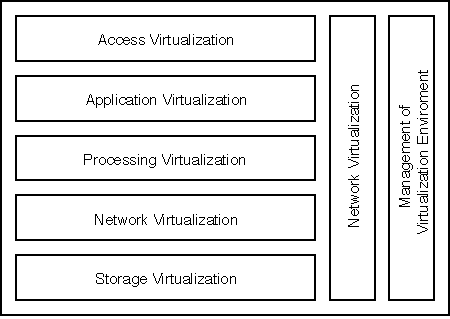
\includegraphics[width=8cm]{images/Kusnetzky2011.pdf}
		\vspace{-0.2cm}
		\caption{Kusnetzky Group model of virtualization \cite{Kusnetzky2011}.}
		\label{fig:kusnetzkyGroupModelOfVirtualization}
	\end{figure}
	
	In 2011, \textit{Dan Kusnetzky} presented the \textit{Virtualization Model of the Kusnetzky Group} \cite{Kusnetzky2011}, which aims to establish a way to organize  virtualizable computing resources, see Figure \ref{fig:kusnetzkyGroupModelOfVirtualization}. The model is composed of seven parts, five of them distributed in the form of layers or levels, located one above the other respectively. Each level represents a type of virtualization in a particular computing environment, such as: \textit{Access}, \textit{Application}, \textit{Processing}, \textit{Network} and \textit{Storage}. The two remaining parts correspond to the \textit{Security} and the \textit{Management} classes, arranged in parallel to the layers above. Below, each of them is briefly described:

	\textbf{Access virtualization} refers to the hardware and software that facilitate access to an application, making it possible for many users to share the same system.
		
	\textbf{Application virtualization} refers to software that allows applications to run transparently on different operating systems and hardware platforms.
		
	\textbf{Processing virtualization} includes the hardware and software elements that allow the division of resources (a system that appears to be many) or the aggregation of resources (many systems that appear to be one).

	\textbf{Network virtualization} refers to hardware and software technologies that make it possible to present a logical view of the physical network elements. This layer can be used for security and multiplexing purposes.
		
	\textbf{Storage virtualization} refers to hardware and software technologies that hide the location and type of physical storage devices in which applications store their data.
		
	\textbf{Security for virtual environment} refers to a set of software elements that make it possible to control access to the various elements of virtual media to protect them from unauthorized actions.
		
	\textbf{Management of virtual environment} refers to the software that makes it possible to performed the administrative and unified management of the available physical resources and the generated virtual environments.

	Although the \textit{Kusnetzky Group model of virtualization} presents a way to include categories for a range of virtualizable computational resources, the model does not provide a good level of detail about the existing technologies in each layer defined in the model. In addition, it does not differentiate between technologies of the same layer. For example, in the \textit{Processing virtualization} there is no evidence of a difference between the types of VMs present in Type-1 or Type-2 hypervisors. 
	
	It is important to note the date of the study and bear in mind technologies which have subsequently been developed. 
